\documentclass[twoside,a4paper,12pt,english]{inac19}

%INAC2019 SETUP: SET PAGE SIZE AND SET FOR USING graphicx PACKAGE.
\usepackage{graphicx}
\usepackage{babel,varioref,epsfig} %,rotating}
\usepackage{amssymb}
\usepackage[font=bf,center]{caption}
\usepackage{subfigure}

\usepackage{textcomp}             % Para usar marca registrada

\title{THE LTHN COMPUTER CLUSTER}

%INAC2019 SETUP: SPECIFY AUTHOR NAMES, AFFILIATION, ADDRESS AND E-MAIL.

%\author
%  {{\bfseries{\normalsize Vitor Vasconcelos A. Silva$^{1}$, Graiciany P. Barros$^{1}$}} \\
%  {\bfseries{\normalsize {Andr\'e A. C. dos Santos$^{1}$}} \\ \\
%    $^{1}$Centro de Desenvolvimento da Tecnologia Nuclear (CDTN/CNEN)\\
%    Av. Presidente Ant\^onio Carlos, 6627 \\
%    31270-901 Belo Horizonte - MG\\
%    vitors@cdtn.br, graiciany.barros@cdtn.br, aacs@cdtn.br\\ \\
%    $^{2}$Departamento de Engenharia Nuclear - UFMG \\
%    Universidade Federal de Minas Gerais\\
%    Av. Presidente Ant\^onio Carlos, 6627 \\
%    31270-901 Belo Horizonte - MG\\
%    }
\author{
  \bf{Vitor Vasconcelos, Andr\'e dos Santos}\\
  \bf{and Graiciany Barros}\\ \\
  CDTN - Centro de Desenvolvimento da Tecnologia Nuclear\\
  Av. Ant\^onio Carlos 6627 - Campus UFMG\\
  31270-901 - Belo Horizonte, MG\\
  \{vitors, aacs, graiciany.barros\}@cdtn.br}



\begin{document}

%INAC2019 SETUP: PRINT TITLE
\maketitle

% Acrescentado para facilitar a redação da NI associada
%\tableofcontents
%\tableofcontents


%INAC2019 SETUP: SETUP HEADS FOR PAGES
\pagestyle{myheadings}
\thispagestyle{empty}
\markboth{}{}


%INAC2019 SETUP: SET FIRST PAGE WITH NO PAGE NUMBER
\thispagestyle{empty}

%--------------------------------------------------------------------------------------
\begin{abstract_full_paper}
In 2024 the LTHN cluster completed 5 years of operation. There were productive five years, in which
the equipment proved itself invaluable for the research work carried on by the LTHN membres and all
the external members with access to the machine. However, in five years a lot can happen - including
a worldwide pandemic - and the cluster suffered from the effects of time. A couple os SSDs failed,
limited software updates due to the lack of personal and changes on the network of the insitute
where the LTHN cluster is located, among less specific but also detrimental small software failures,
caused a degradation of the service. Less machines operating, ocasional loss of data and problems
on the scheduler were the main problems users of the system faced when running their jobs. With that in
mind, a major updated of the system was carried on and is the subject of this paper, which will
present the main changes and updates made to the system on its sixth year of operation. These changes
are carefully described and will hopefully be of good use for small clusters users and admins. We also
present the performance of the updated system for heavier and more complex simulations run currently
on the LTHN cluster.
\end{abstract_full_paper}

%--------------------------------------------------------------------------------------
\section{INTRODUCTION}\label{int}

This paper presents the current situation of the LTHN/CDTN (Thermal-hydraulics and Neutronics
Laboratory/Nuclear Technology Development Center) computer cluster. This cluster is the main 
computational tool of the research group and it is mainly used on Neutronics and Thermal-hydraulics 
numerical simulations. In this work it is briefly described, considering hardware and software, 
with special focus on the software solutions which allows its operation on a 24/7 basis.

The present work is a follow-up, considering the natural degradation of a complex computer
equipment, of the work carried on by the same team presenting the use and characteristics
of the LTHN computer cluster\cite{cluster19}.

%------------------------------------------------------------------------------
\subsection{Context}

It is probably unnecessary to mention the importance of computers to all the work carried on 
in the field of Science and Technology. Put shortly: the magnitude of calculations and simulations 
achieved using computers - in this case, a special set of them - are simply impossible without 
them and this fact makes computers integral part of scientific development. An elegant outlook 
on this matter is given by Dongarra\cite{Dongarra2017}.

%------------------------------------------------------------------------------
\section{OBJECTIVE}

The objective of this work is to present the current status of the cluster equipment 
at the Laboratory of Thermal-hydraulics and Neutronics of CDTN (\textbf{LTHN}), describing the decisions 
taken during the installation process, the solutions applied to common (and uncommon) problems 
derived from running a professional cluster system. Together with technical decisions, the 
performance of the system is asserted by comparison to the older system used by the laboratory 
team. 


%------------------------------------------------------------------------------
\section{METHODS AND PROCEDURES}


%------------------------------------------------------------------------------
\subsection{Network}


\subsection{Hardware}

The \textit{slaves} are Dell workstations Precision R7910 equipped
with Dual Intel{\textregistered} Xeon{\textregistered} processors E5-2640 operating at $2.4$GHz with
$32$Gb of RAM each. They have two $10$GbE (Gigabit Ethernet) and also two $1$Gbit network connectors, which
allow the use of the Gigabit network exclusively for intra-cluster communication. Their disks are $360$Gb SSD
and are used to store the Operating System of each node and also part of the \textit{Gluster} distributed
file system. These equipments are also installed with Nvidia{\textregistered} GPUs (Graphic Processing Units) M4000{\textregistered} with $8$Gb CUDA\cite{CUDA} capable.

\begin{figure}[h] % t forces top and b forces bottom: can be added to h, ex. [ht]
  \centering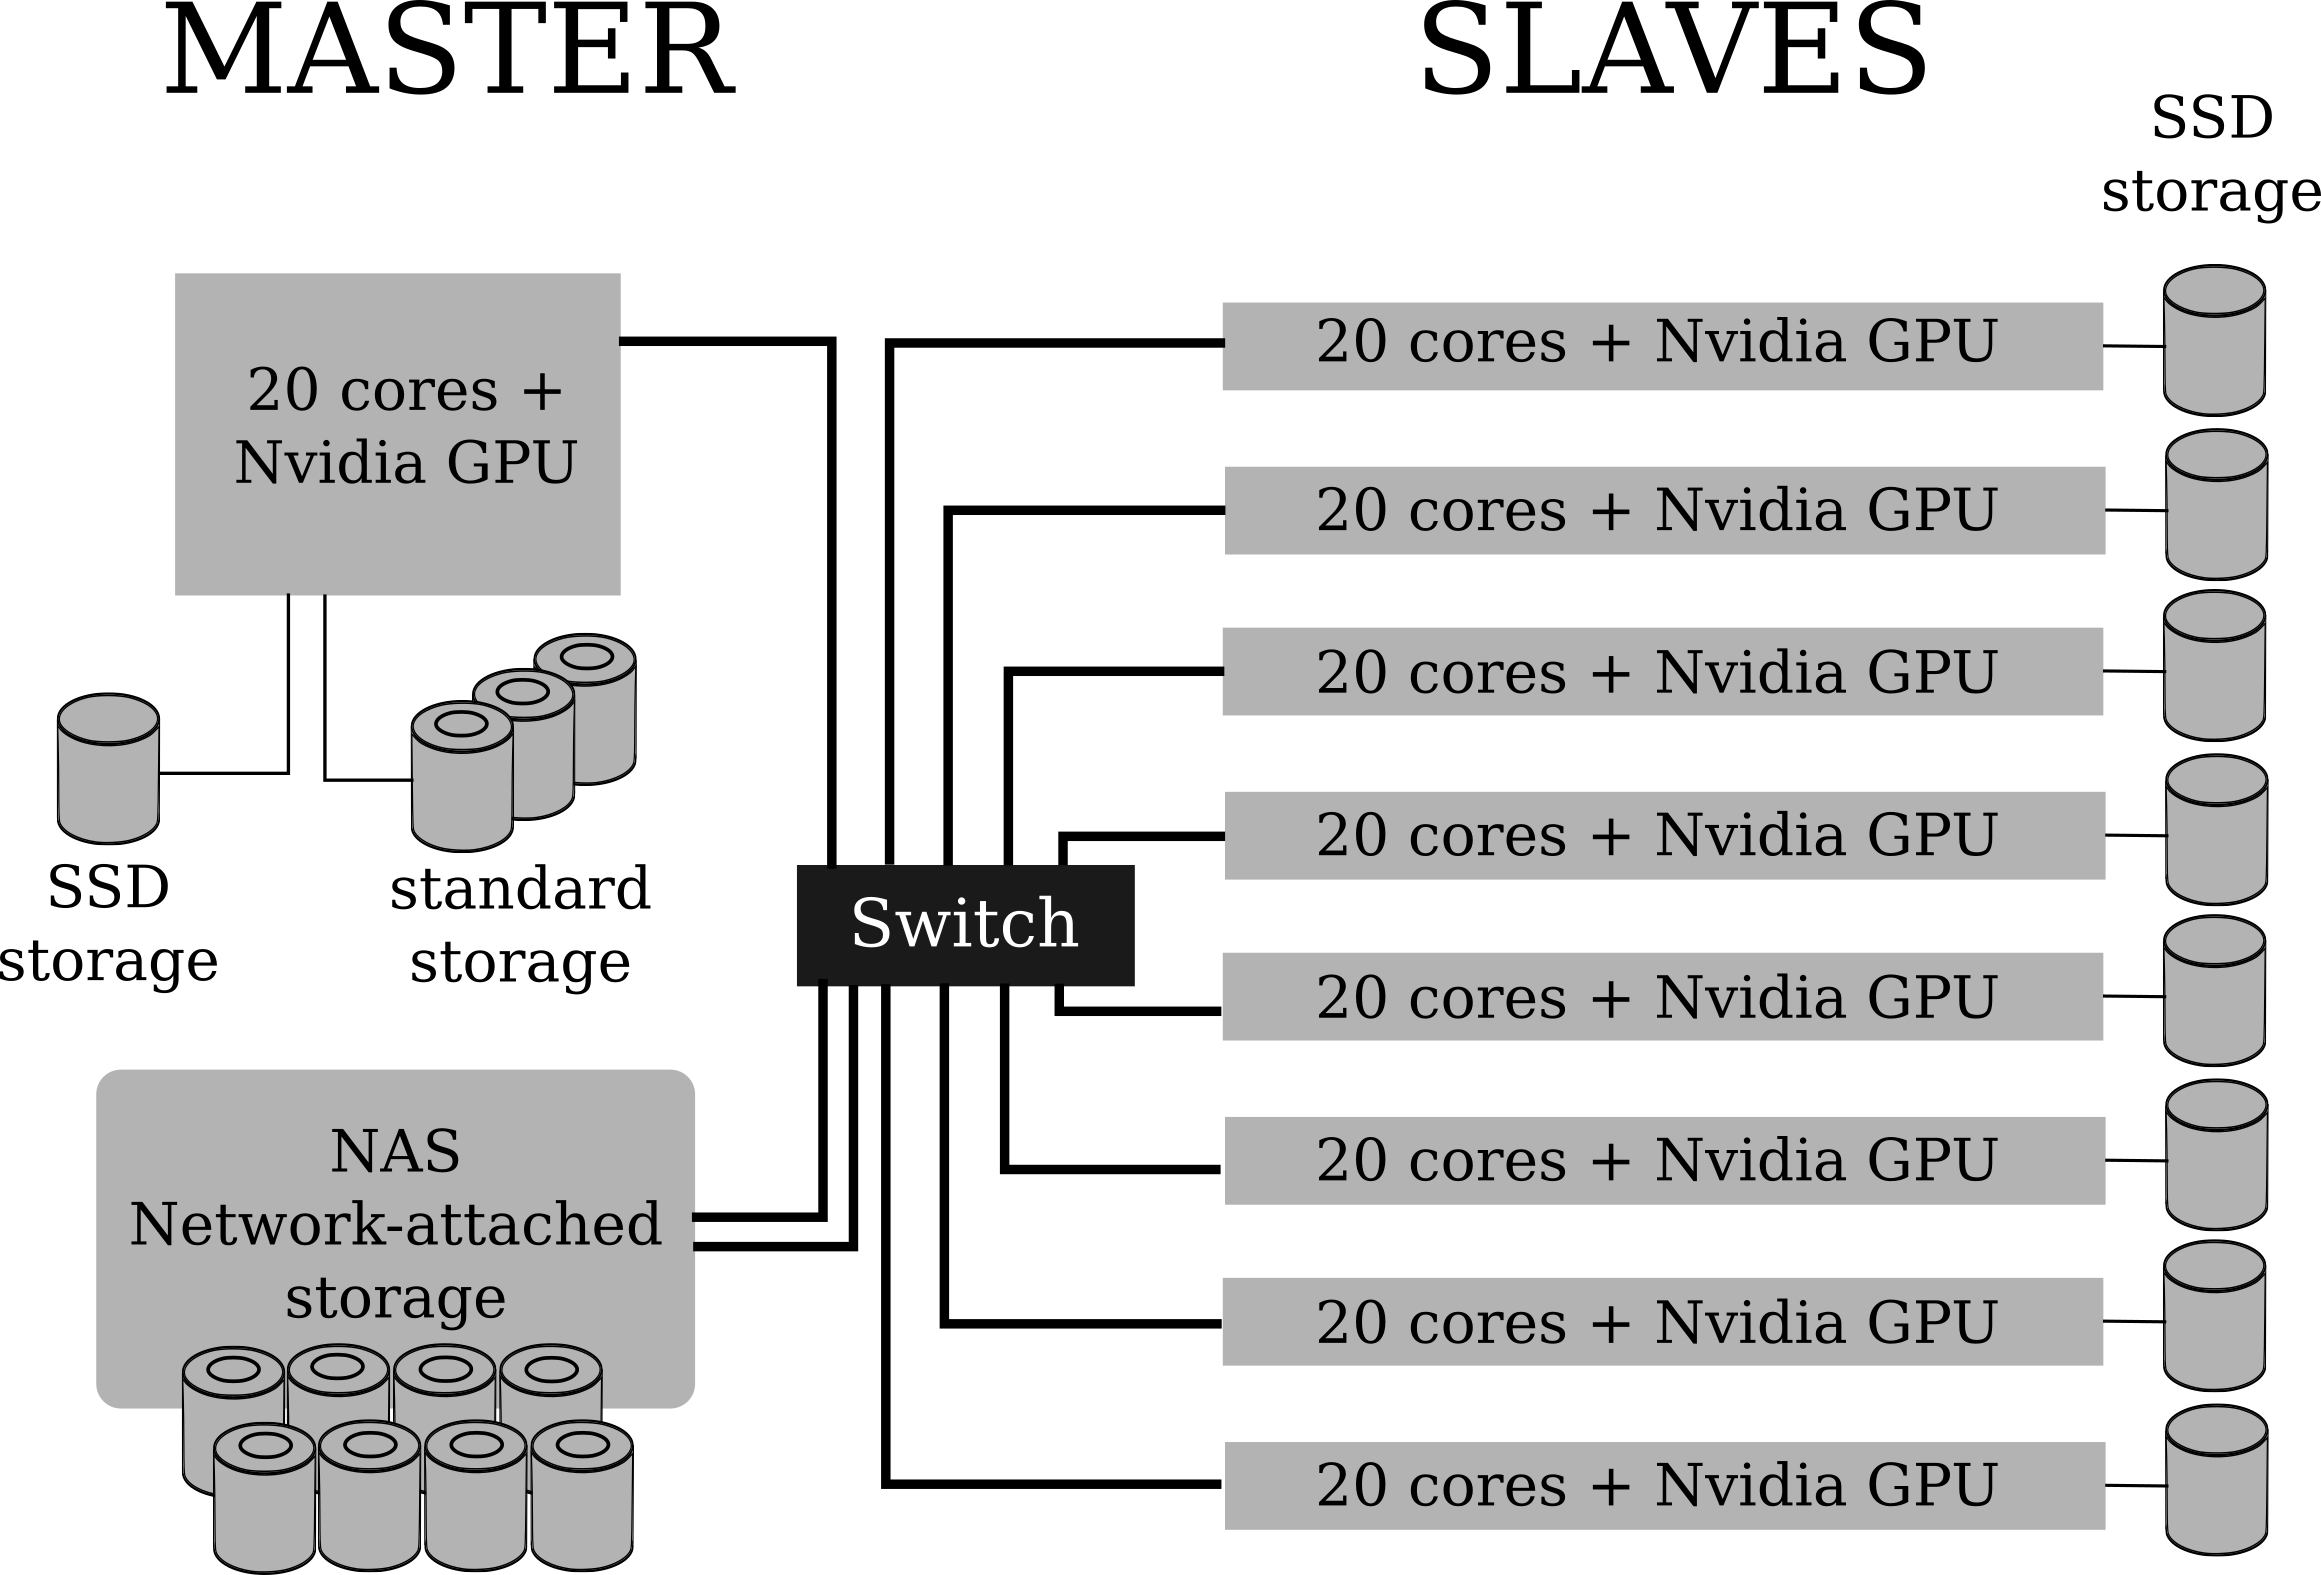
\includegraphics[scale=0.7]{images/cluster-topologico.png}
  \caption{Cluster hardware.}
  \label{fig:cluster}
\end{figure}

The GPUs on nodes are used as calculation units by the software which can take advantage of this kind of hardware.
The use of hardware acceleration in scientific computing is not new and have been increasing consistently on the
last years\cite{accelerators}.

The \textit{master} node is a Dell Precision T7910. The main
differences between the \textit{master} node and the \textit{slaves} machines are two: the \textit{master} has
a slightly worst graphics card, a Quadro{\textregistered} M2000 with $4$Gb of memory. However, the second difference
is the amount of RAM memory. The nodes are equipped with $32$Gb of memory whereas the \textit{master} has
$256$Gb of RAM.


Three hard-disks of $500$Gb are physically connect to the \textit{master} node and are used as part of the 
\textit{Gluster} distributed file system, offering
an extra $1.5$Tb of storage for the whole system.


%--------------------------------------------------------%

%------------------------------------------------------------------------------
\subsubsection{NAS}

NAS (Network Attached Storage) is a computer data storage server connected to a computer
network with the objective to serve files for the computers attached to this network. This
dedicated hardware is used in the cluster system to provide a directory where users accounts
are kept. The system used is a NAS Synology DS1817, using its proprietary DSM system, version
6.2.1 and has 4Gb RAM. It is equipped with 8 identical hard-disks, each one of 3.7 Tb of space.

Internally, the system is configured with two volumes, both operating as RAID 10,
which means that data is replicated and that only half of the whole available space
can be used since the other half mirrors the data as a backup, making the total
of 7.21 Tb available at each volume.

The space where the users accounts are kept is mapped as NFS (Network File System) at the
cluster itself and quotas are kept to avoid system malfunction due to poor resources management
by the users.

The NAS is connected to the cluster system trough a bond connection. The bond connection is a logical
connection which uses two 10 Gbits connection to improve traffic band and is completely hidden from
the cluster system, which ``sees'' a 20 Gbits connection and one IP address.


%------------------------------------------------------------------------------
%\subsection{Applications}
%\label{sub:apps}


%------------------------------------------------------------------------------
\subsection{Software Solutions}
\label{sub:ssol}


It is worth mention that among the main software solutions a simple and yet powerful package 
allows the use of embedded temperature monitoring hardware to display system's temperature. 
Although now only used on system administrator needs, it can be used to automate system's 
responses in specific events. Of course, on top of the already available operational systems 
safety measures. 

%------------------------------------------------------------------------------
\subsection{File System}

During the installation phase of the cluster system there were two the contenders for
distributed file system solution. The chosen one is described below.

%------------------------------------------------------------------------------
\subsubsection{Gluster File System}

GlusterFS\cite{gluster} is an open source, distributed file system and has
a unique no-metadata server architecture. This is the chosen solution for the system due to its relatively
small number of physical disks and nodes (nine).

\begin{figure}[ht] % t forces top and b forces bottom: can be added to h, ex. [ht]
%  \centering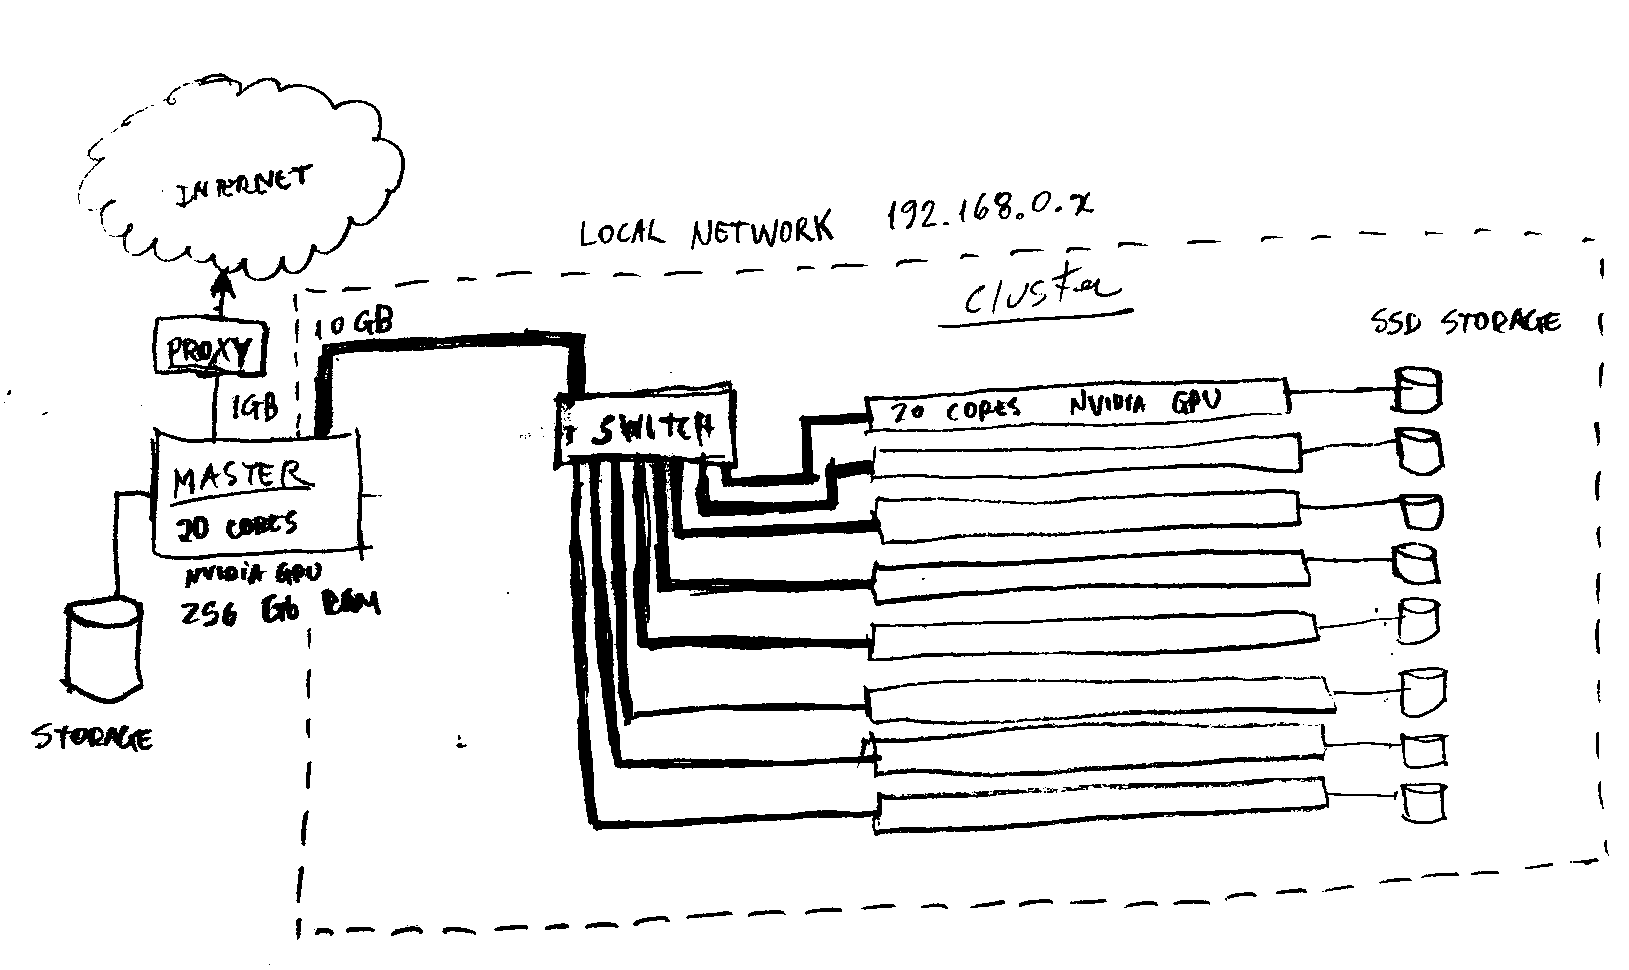
\includegraphics[width=8.5cm,height=8.5cm]{images/esquema_cluster_edited_bw.png}
  \centering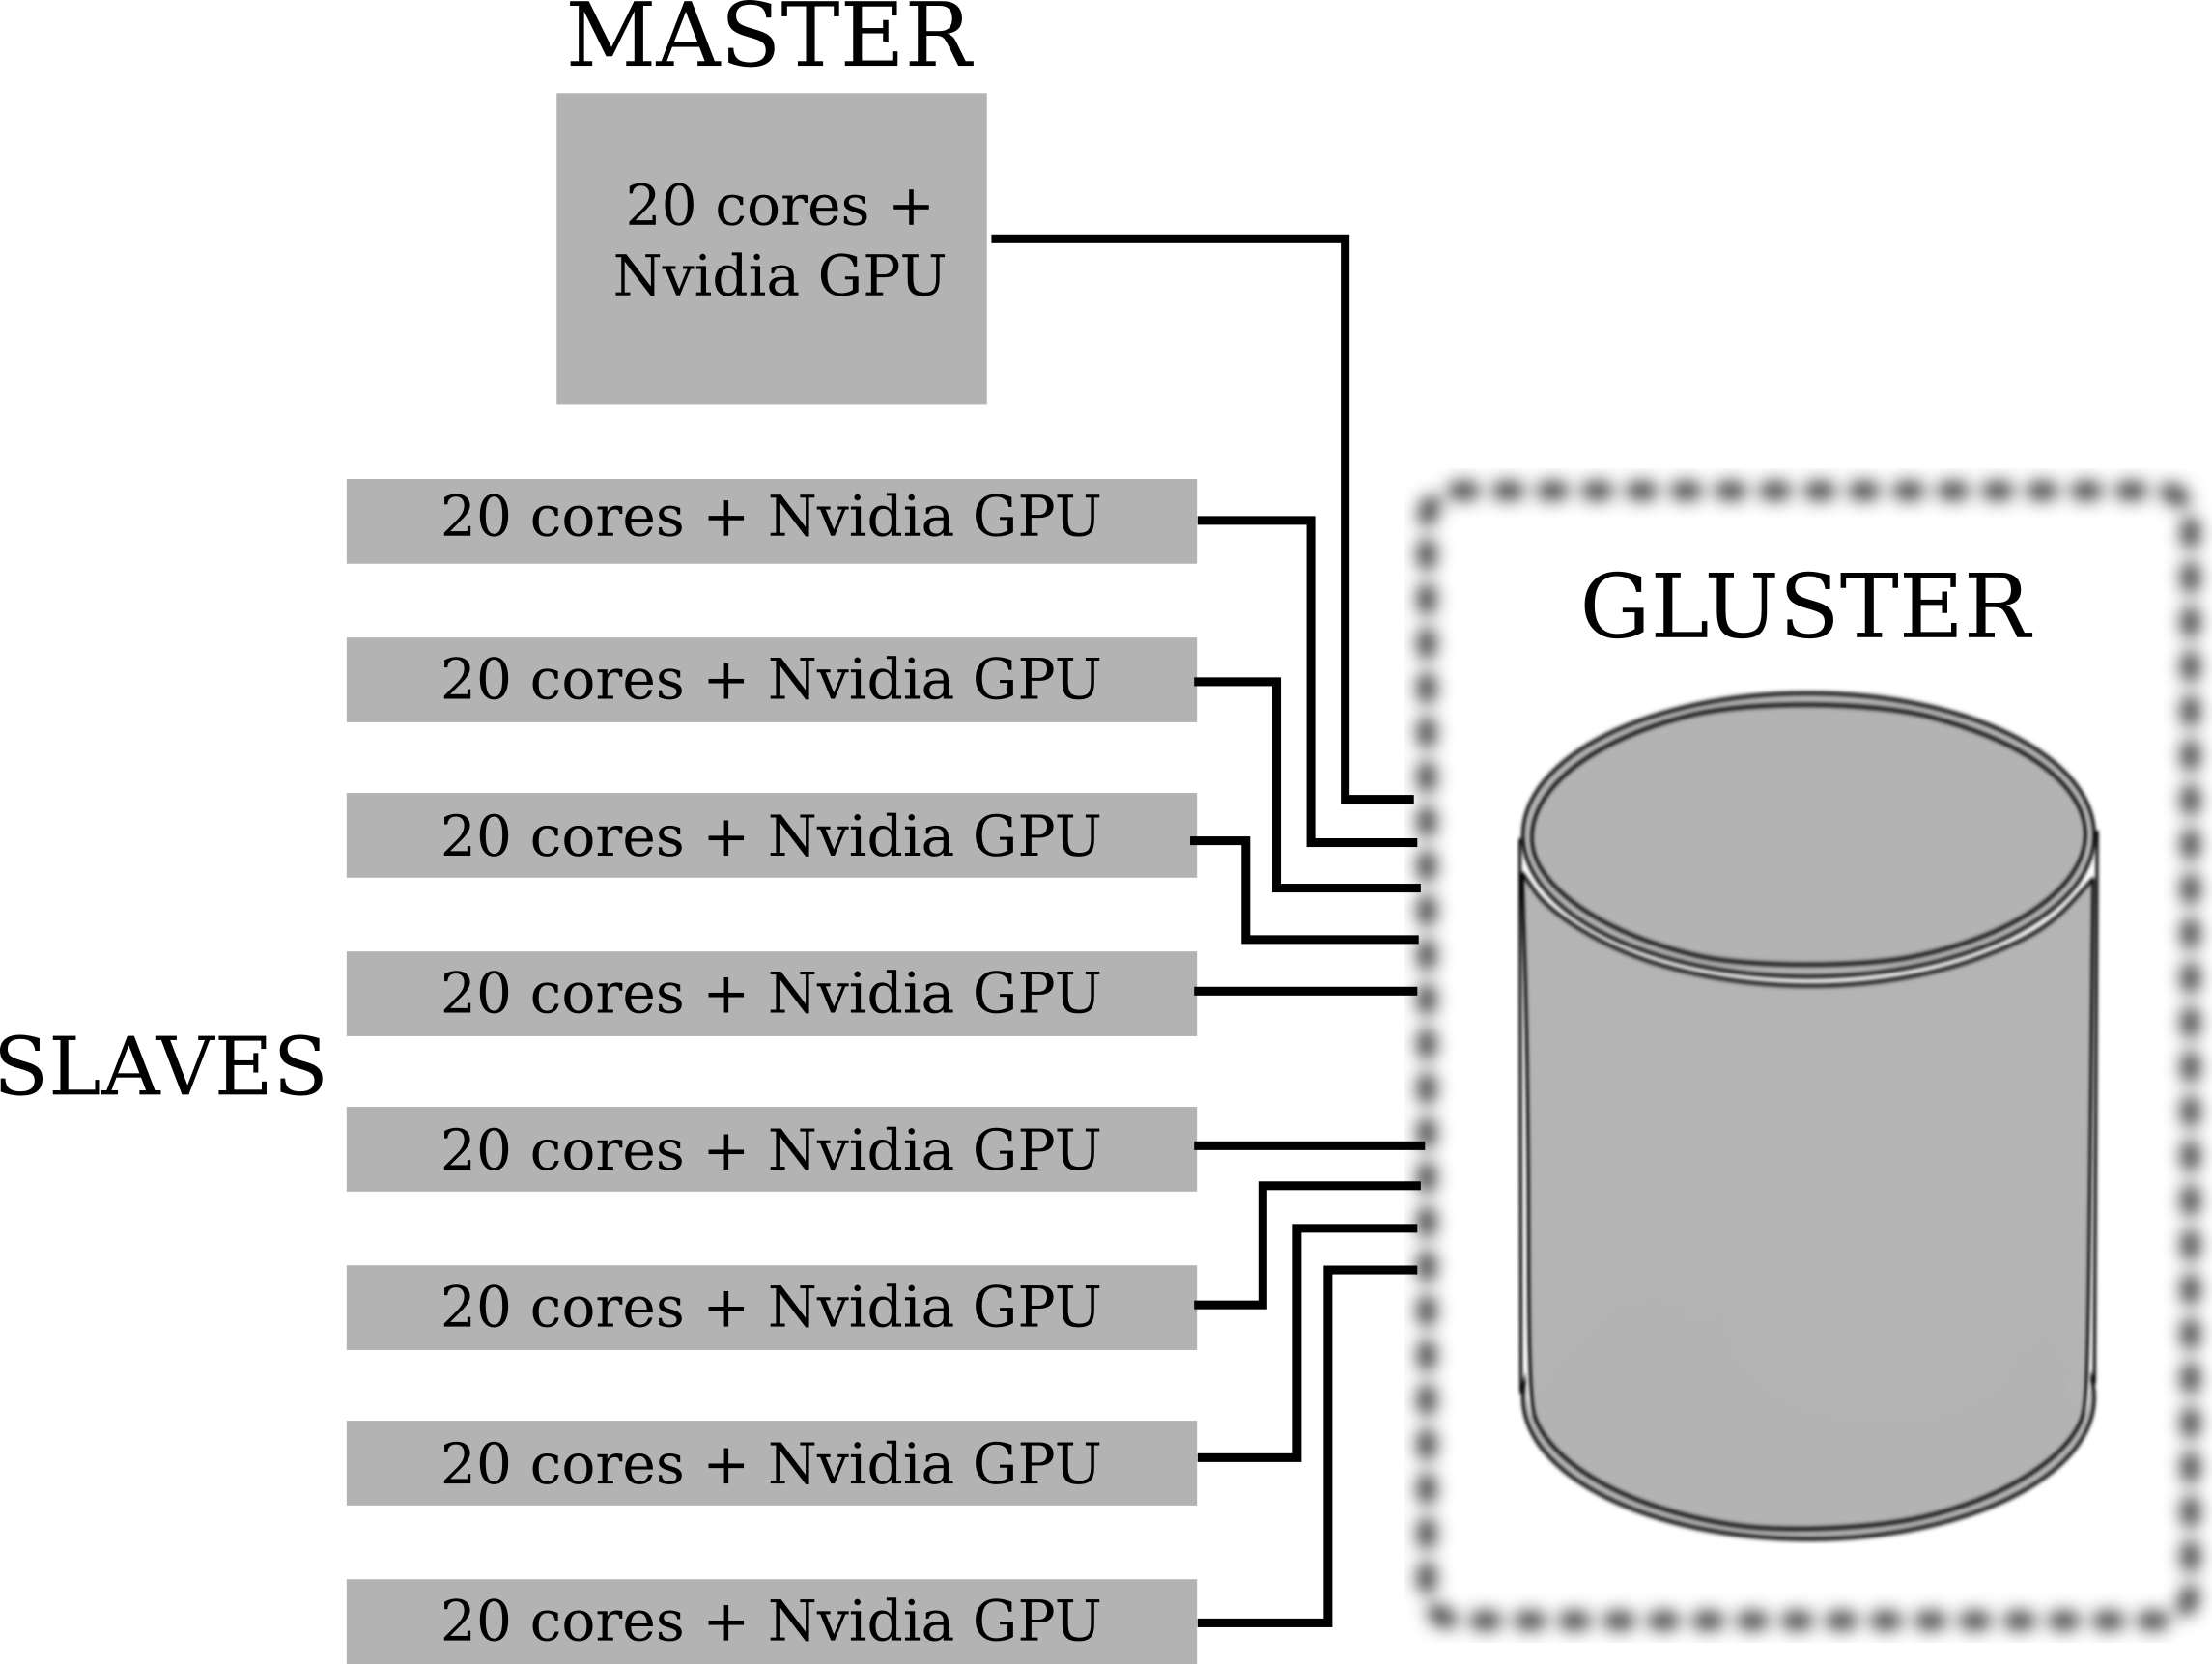
\includegraphics[scale=0.7]{images/cluster-gluster.png}
  \caption{``View'' of \textit{Gluster} distributed file system.}
  \label{fig:cluster-gluster}
\end{figure}

The system is configured to use two \textit{gluster} volumes, namely \texttt{gv-apps} and \texttt{gv-data}. Both volumes
are configured as \textit{distributed} without replication. Since the whole system has an extra NAS device, there is
no need of keeping redundant data. The \texttt{gv-data} offers $N$ Gb of storage per user and is used to run simulations or any task that needs storage during execution. After that, data must be moved to a storage space on NAS where an automatized regular backup avoids data loss.

Figure \ref{fig:cluster-gluster} shows the "software" view of \textit{gluster} by the system's operational system. The big 
gluster disk is, in reality, a set of different hard disks grouped in the mentioned volumes and controlled by the 
\textit{gluster} daemons running on each node and the control daemon running only on the master node.

%------------------------------------------------------------------------------
\subsection{Job scheduler}
\label{ssec:slurm}

\textit{Slurm}\cite{slurm} is an open source and scalable workload manager, widely used for large
and small - the present case - Linux clusters. It is transparent to the kernel, needing no changes in
kernel modules to fully work.

Its architecture is relatively simple, having a centralized manager called \texttt{slurmctld} responsible for
monitoring resources and workload. Each node has a daemon called \texttt{slurmd} which is responsible for
wait for and execute work, return status and communicate to the manager. An optional database daemon
(\texttt{slurmdbd}) can be used to record account information. This database is installed in the cluster
system described in this paper.

Together with daemons, \textit{Slurm} provides a set of commands which are the interface between users
and the scheduler, used by the users to run, check, cancel and control theirs jobs. A glimpse of \textit{Slurm}
architecture is presented in Figure \ref{fig:slurm}.

\begin{figure}[h] % t forces top and b forces bottom: can be added to h, ex. [ht]
  \centering\includegraphics[scale=0.5]{images/slurm-arch.png}
  \caption{Slurm architecture. (Source: Slurm website)}
  \label{fig:slurm}
\end{figure}

\subsubsection{System use: basics}
The access to the cluster system is made as simple as possible. However, the absence of a Graphical User Interface
(GUI) slightly increases system's difficult of use, specially for those not used to command line. That said, only
a handful of commands are necessary to login, check jobs queue and submit a job. System's login screen is shown
in Figure \ref{fig:login-screen}.

\begin{figure}[h] % t forces top and b forces bottom: can be added to h, ex. [ht]
  \centering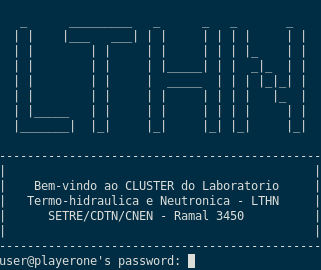
\includegraphics[scale=0.7]{images/p1login.png}
  \caption{LTHN cluster login screen.}
  \label{fig:login-screen}
\end{figure}

Of course, a basic understanding on how to use Linux shell can be of great value of productivity for users.
Those users with basic knowledge on shell scripting are the best served as they will be able to fine tuning
their simulations through scripts. That said, a basic recommendation to all users is to carefully read and
study Chapter 1 and 2 of reference\cite{ECP}.

%------------------------------------------------------------------------------
\subsection{System monitoring tool}
\label{ssec:ganglia}

At this point it is clear the importance to be able to submit jobs, have them scheduled following priorities
and having a load balancing scheme to help optimizing the cluster's resources. Nonetheless, the ability to
monitor and check system's load on different nodes, taking account different resources - memory, disk, IO,
etc. - without the need to log in to the system is, at the minimum, practical.

This fundamental task is accomplished by \textit{Ganglia}\cite{ganglia}, a monitoring system built in
a modular design which offers a web interface to access monitoring data. Figure \ref{fig:ganglia-rainbow} shows
one of the graphics provided by default by it. In this example, the relative load of nodes is show in time,
one color by node.

\begin{figure}[th] % t forces top and b forces bottom: can be added to h, ex. [ht]
%  \centering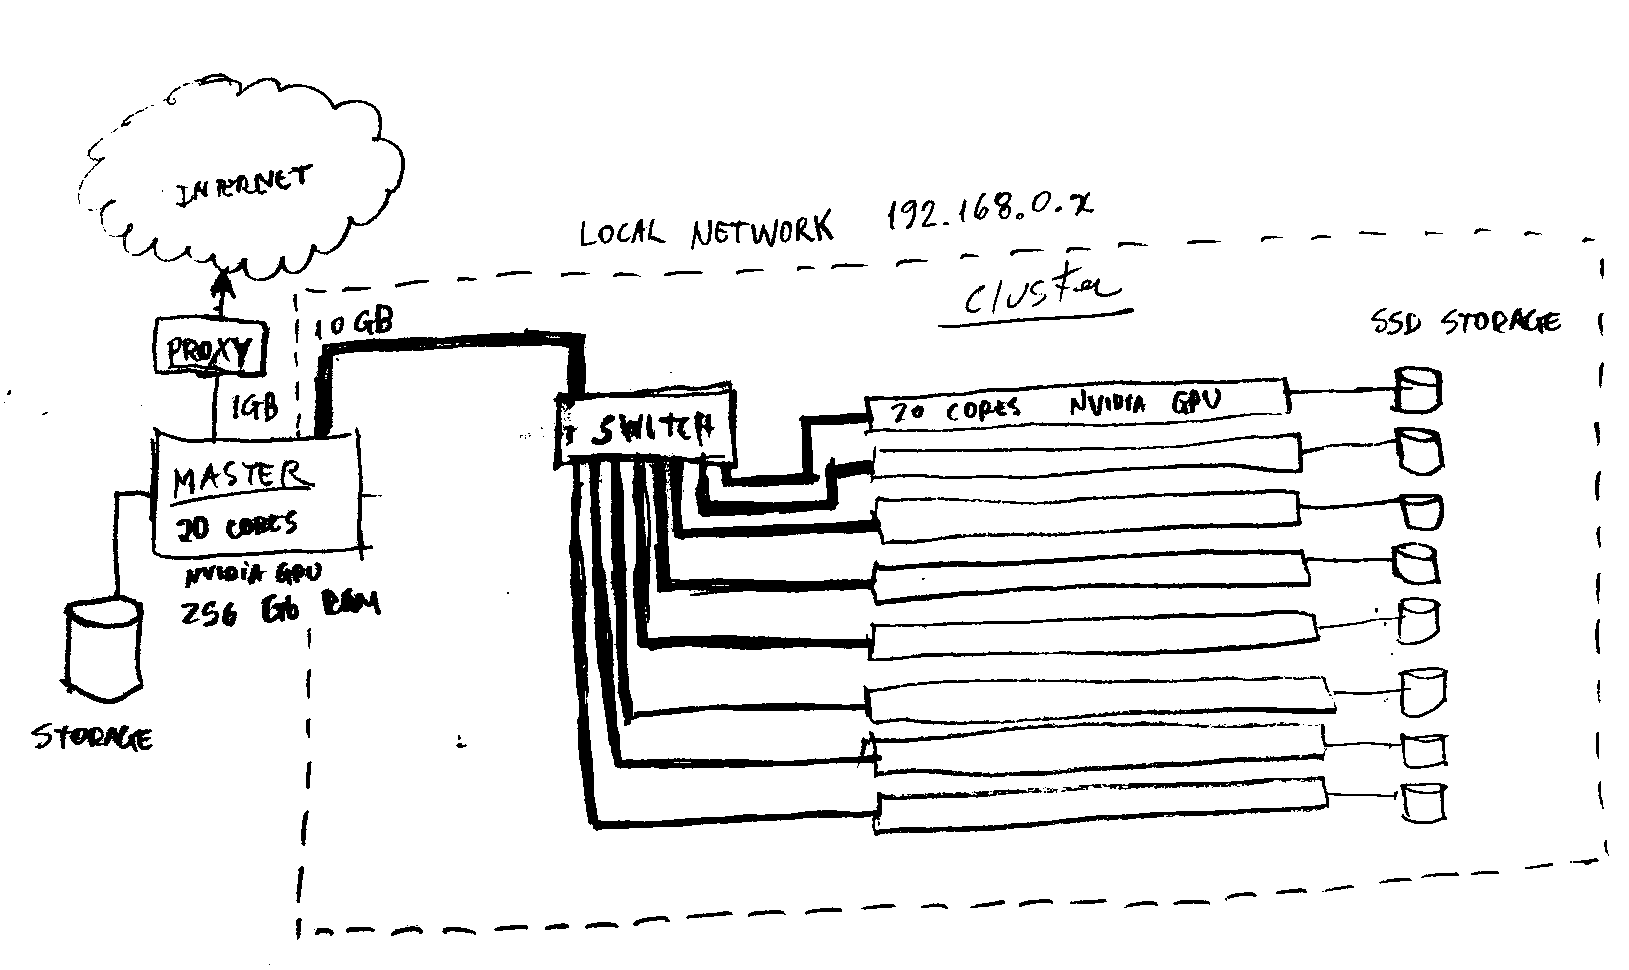
\includegraphics[width=8.5cm,height=8.5cm]{images/esquema_cluster_edited_bw.png}
  \centering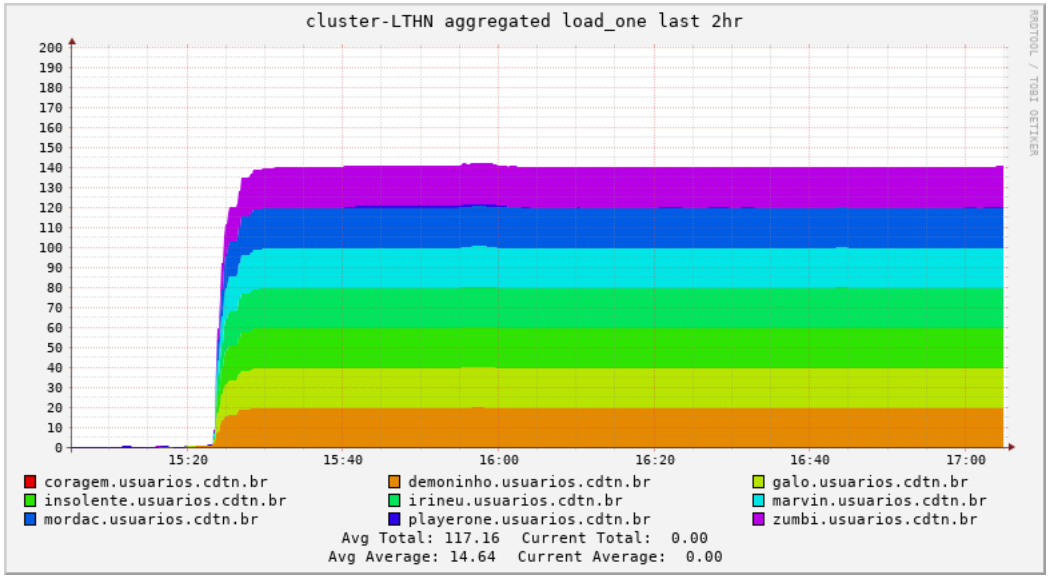
\includegraphics[scale=0.55]{images/ganglia_rainbow.png}
  \caption{A color graphic showing relative node use.}
  \label{fig:ganglia-rainbow}
\end{figure}

The architecture of \textit{Ganglia} is out of the scope of this paper, but can be said that it has metadata
daemons working in multicast mode. In other words, every node collects and shares information with one or
more monitors - the cluster system only uses one - which shares this information by the use of a web server.
So, all data, as configured by the system administrator, can be checked by any user with access to the
web server.

It is worth mentioning that the type of data collected can be extended by the use of modules. The development
of new modules is done using an API (Application Programming Interface) based on Apache web server API\cite{apache}
and no changes to \textit{Ganglia} have to be done: the module can be simply loaded by it.

%\begin{figure}[h] % t forces top and b forces bottom: can be added to h, ex. [ht]
%  \centering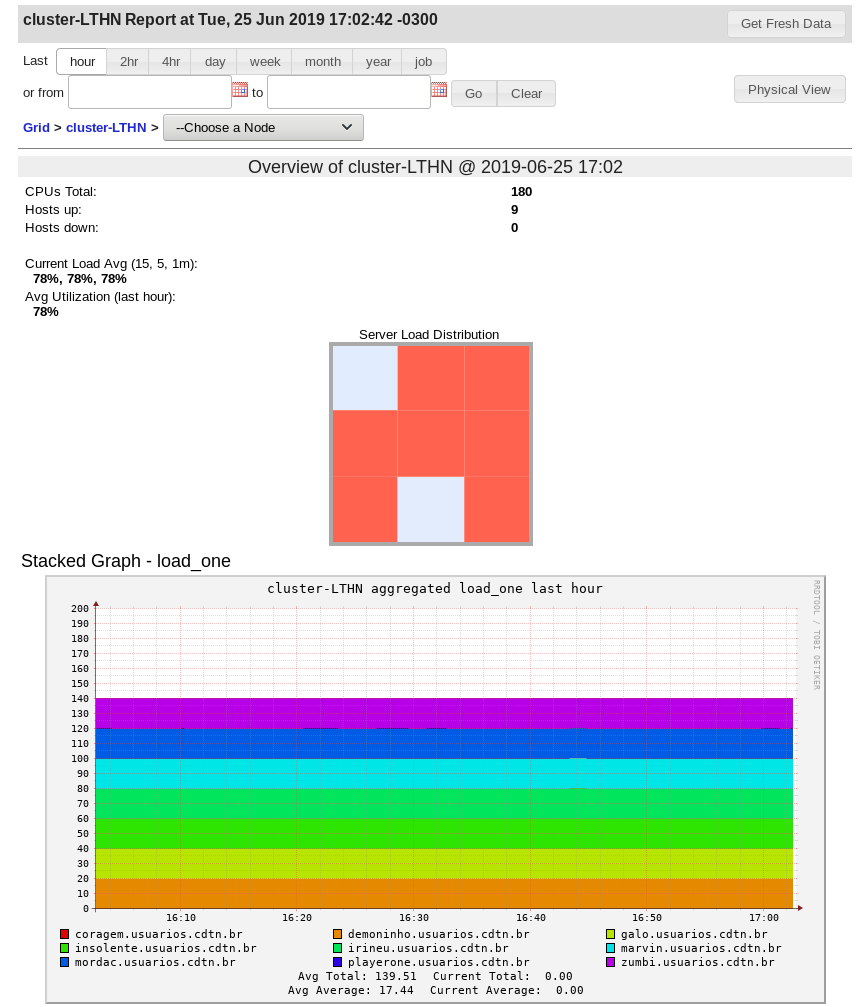
\includegraphics[scale=0.7]{images/ganglia_colors.png}
%  \caption{Color reference screen showing nodes loads.}
%  \label{fig:ganglia-colors}
%\end{figure}

%\begin{figure}[h] % t forces top and b forces bottom: can be added to h, ex. [ht]
%  \centering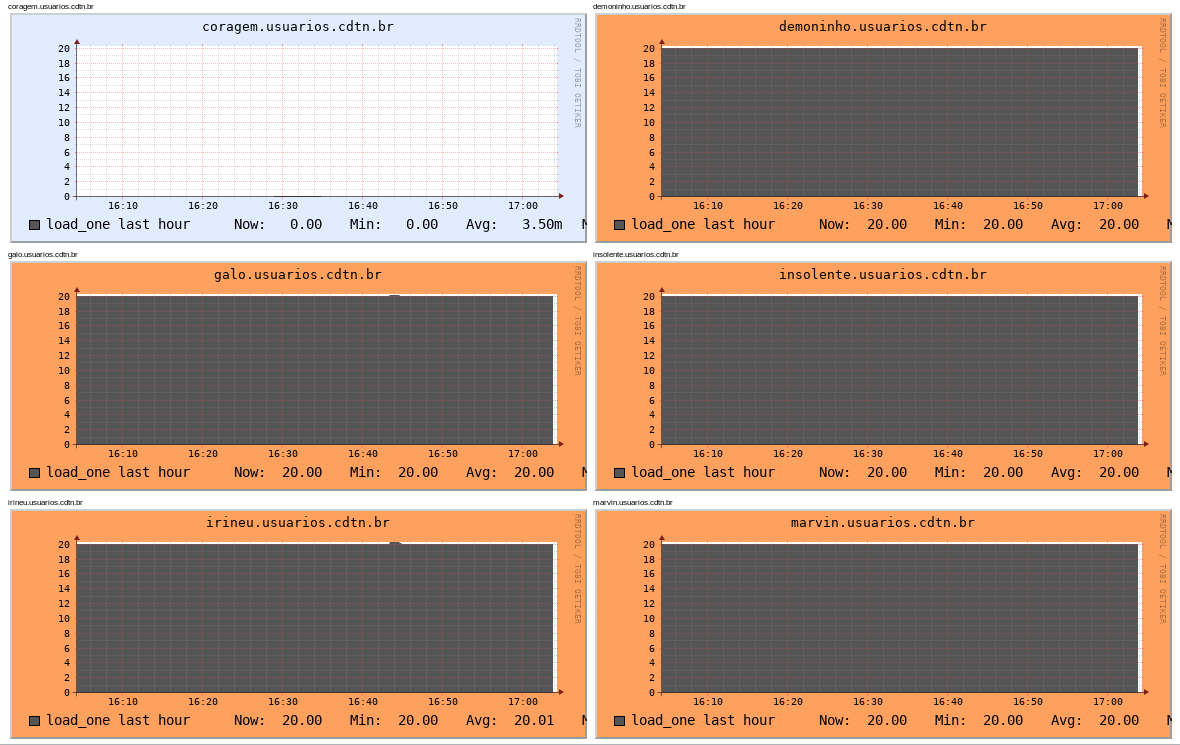
\includegraphics[scale=0.5]{images/ganglia_nodes.png}
%  \caption{Nodes load on the monitoring system.}
%  \label{fig:ganglia-nodes}
%\end{figure}

%------------------------------------------------------------------------------

\section{RESULTS AND ANALYSIS}

At the time of writing these lines, the system is up and running non-stop for 93 days. This is a
basic measurement of it robustness. A total of $907$ jobs were submitted since the installation
of the scheduler, including failing jobs,
test jobs and also working cases jobs. The bulk of most submitted jobs are thermal-hydraulics
simulations using ANSYS CFX and ANSYS Fluent. Only a part of all simulations are related to neutronics.
There is no special reason for this bias in favor of thermal-hydraulics than the recent need of the users.
%The reason for that is fairly simple: the workflow is completely dictated by the needs of users
%and during the last 2 months of system monitoring most sheduled works were from students of mechanical
%and aerospatial engineering finishing their final undergraduation works.

In order to present some quantitative results two neutronics problems were modelled. The hardware used
to run these problems is:

\begin{itemize}
\item Desktop: Intel(R) Xeon(R) CPU E5520 @ 2.27GHz, 8 CPUs, 48Gb RAM.
\item Nodes: Intel(R) Xeon(R) CPU E5-2640 v4 @ 2.40GHz, 20 CPUs, 32Gb RAM.
\end{itemize}

The number of available nodes is 8, although not used for both simulations.

One simulation was run using Serpent Nuclear code, installed in both the cluster and desktop machines at the Thermal-Hydraulics
and Neutronics Laboratory (LTHN), version 2.1.31 compiled to make use of OpenMP\cite{openmp}. This simulation involves burning
significative number of different isotopes and is considered the heavy test presented in this work. It is worth mentioning
that, due to lack of a proven thread-safe MPI implementation, the compiled version of Serpent runs only in one machine.
This translates to the maximum of one node running on its full: 20 processors.

The results of the this benchmark are presented in Table \ref{table:benchmark-serpent}.

\begin{table}[ht]
  \caption{Serpent benchmark}
  \centering
\begin{tabular}{c|c|r}
Machine & \begin{tabular}[c]{@{}c@{}}Number\\ of processors\end{tabular} & \multicolumn{1}{c}{\begin{tabular}[c]{@{}c@{}}Elapsed\\ time\end{tabular}} \\ \hline
Desktop & 8                                                              & 00:21:34                                                                   \\
Node    & 8                                                              & 00:12:46                                                                   \\
Node    & 20                                                             & 00:05:12                                                                   \\
Node    & 160                                                            & 00:00:42                                                                  
\end{tabular}
\label{table:benchmark-serpent}
\end{table}

The second benchmark uses MCNP6 and is a fairly simple simulation, consisting in simulating the response in dosis
to a set of detectors scattered in surfaces in a room with a defined radiation source. This model
was run using 8 processors (the maximum available at the desktop machine) in both desktop
and node, plus 20 processors and 160 processors in the cluster.

The results of MCNP simulations are shown in Table \ref{table:benchmark-mcnp}.

\begin{table}[ht]
  \caption{MCNP benchmark}
  \centering
\begin{tabular}{c|c|r}
Machine & \begin{tabular}[c]{@{}c@{}}Number\\ of processors\end{tabular} & \multicolumn{1}{c}{\begin{tabular}[c]{@{}c@{}}Elapsed\\ time\end{tabular}} \\ \hline
Desktop & 8                                                              & 2 days, 08:26:43                                                                   \\
Node    & 8                                                              & 1 day, 11:02:36                                                                   \\
Node    & 20                                                             & 23:19:46                                                                   
\end{tabular}
\label{table:benchmark-mcnp}
\end{table}


%------------------------------------------------------------------------------

\section{CONCLUSIONS AND PERSPECTIVES}

The LTHN cluster works with robustness, being up for 93 days non-stop at the time of this writing.
It is used without issues by a group of about 10 users. That said, some improvements are envisaged, most
of them external to the cluster itself.

The environmental one is to automatize power monitoring by means of connecting a software monitor systems to
the no-break and power supplies of the system, adding the ability to the system to shutdown in case
of a likely to happen power outage. A similar project concerning the air-conditioning system is envisaged,
by the use of a single board computer and temperature sensors.

However, the main work on cluster improvement is to take advantage of the GPUs (Graphics Processing Units) to
visualize data. Two options are under consideration: one is the use of VirtualGL\cite{virtualgl}. It is an
open source toolkit that gives to Linux and Unix remote display software the ability to run OpenGL applications
with full hardware acceleration. The limitation of this approach is that machines running other operating
systems will not be able to take advantage of remote visualization. The other option is to make use of
Paraview\cite{paraview} in client-server mode. Instances of paraview server would run on nodes and
locally use GPUs to render data. These data is then accessed by paraview clients running on ordinary machines,
with no need of special hardware. Both options are under study and, decision made, the implementation of the
solution will be probably done on the first half of 2020.


%Uma cita\c{c}\~{a}o \cite{Henderson17}.


%------------------------------------------------------------------------------



\section*{Acknowledgments}
The authors would like to thank FUJB for financing the cluster acquisition
as part of the project \textit{Desenvolvimento de novos elementos combust\'{i}veis nucleares
  e materiais e pe\c{c}as para combust\'{i}veis nucleares}, agreement FINEP 01.07.0548.00 - Process FUJB 13.867-3.
The authors also thank Dr. Jo\~{a}o Roberto Loureiro de Mattos, now retired, for the work which made possible the acquisition of the cluster.

%%%%%%%%%%%%%%%%%%%%%%%%%%%%%%%%%%%%%%%%%%%%%%%%%%%%%%%%%%%%%%%%%%%%%%%%%%%%%%%%%%%%%%%%%%%%

\begin{thebibliography}{99} %99 é o número máximo que o thebibliography permite. Numero de referencias que aparecerão.

\bibitem{cluster1} MUDAR PARA O PAPER DE 2019 Vitor V. A. Silva, Andr\'{e} A. C. dos Santos and Renan O. Cunha, ``Professional Cluster Management
  by a small scientific team: challenges, solutions and perspectives'', \textit{XX ENFIR INAC 2017 International Nuclear Atlantic Conference }, Belo Horizonte, MG, Brazil, October, (2017). 
  
  %\bibitem{linux} ``The Linux Documentation Project'', \\\verb#http://www.tldp.org/LDP/intro-linux/html/chap_01.html# (2019).
  
\bibitem{Dongarra2017} John Dongarra et. al., ``With Extreme Computing, the Rules Have Changed'', \textit{Computing in Science Engineering}, \textbf{19}, pp. 52--62, (2017).
  
\bibitem{CUDA} John Nickolls, Ian Buck, Michael Garland and Kevin Skadron, ``Scalable Parallel Programming with CUDA'', \textit{Queue - GPU Computing}, \textbf{6}, pp. 40--53, (2008).
  
\bibitem{accelerators} David Tarditi, Sidd Puri, and Jose Oglesby, ``Accelerator: using data parallelism to program GPUs for general-purpose uses'',  \textit{SIGPLAN Not. 41}, \textbf{11}, pp. 325--335. DOI: https://doi.org/10.1145/1168918.1168898 (2006).

\bibitem{gluster} Alex Davies and Alessandro Orsaria, ``Scale out with GlusterFS'', \textit{The Linux Journal}, \textbf{2013}, (2013).

\bibitem{slurm} A. Yoo, M. Jette, and M. Grondona, ``Slurm: Simple Linux Utility for Resource Management'', Job Scheduling Strategies for Parallel Processing, \textbf{2862} of \textit{Lecture Notes in Computer Science}, pp. 44--60, Springer-Verlag, (2003).

  \bibitem{ECP} Anthony Scopatz and Kathryn Huff, \textit{Effective Computation in Physics: Field Guide to Research with Python}, O'Reilly Media, ISBN 978-1491901533, (2015).

  %\bibitem{windows7} Jorge Orchilles, \textit{Microsoft Windows 7 Administrator's Reference}, Syngress, Boston USA (2010).

\bibitem{ganglia} Matt Massie, Bernard Li, Brad Nicholes and Vladmir Vuksan, \textit{Monitoring with Ganglia}, O'Reilly Media, ISBN 978-1449329709, (2012).

\bibitem{apache} Ryan B. Bloom. \textit{Apache Server 2.0: The Complete Reference}, McGraw-Hill, Inc., New York, NY, USA (2002).
  
  \bibitem{openmp} Leonardo Dagum and Ramesh Menon. ``OpenMP: An Industry-Standard API for Shared-Memory Programming'', \textit{IEEE Comput. Sci. Eng.}, \textbf{5}, 1, pp. 46--55, (1998), DOI: https://doi.org/10.1109/99.660313 

\bibitem{virtualgl} ``A Brief Introduction to VirtualGL'', \verb#https://virtualgl.org/About/Introduction# (2019).

\bibitem{paraview} Ayachit, Utkarsh, \textit{The ParaView Guide: A Parallel Visualization Application}, Kitware, ISBN 978-1930934306, (2015).
  
  
%  \bibitem{apache} APACHE.
    
\end{thebibliography}

% ---------------------------------------------------------
% Minha bibliografia usando arquivo externo
%\bibliographystyle{unsrt}
%\bibliography{bibli}


\end{document}
